\documentclass[10pt, t]{beamer}
\usetheme{metropolis}           % Use metropolis theme

\ifnotes
  \hypersetup{final}
  \usepackage{pgfpages}
  \setbeamertemplate{note page}[plain]
  \setbeameroption{show notes on second screen=right}
\fi

\usepackage{appendixnumberbeamer}
\usepackage{algpseudocode}
\usepackage{multirow}
\usepackage{verbatim}
\usepackage{tikz}
\usetikzlibrary{decorations.pathreplacing}
\usepackage[scale=3]{ccicons}   % creative commons icons

\title{Performance analysis}
\date{}
\author{Jeremy Iverson}
\institute{College of Saint Benedict \& Saint John's University}

\begin{document}

  \begin{frame}
    \titlepage
  \end{frame}

  \begin{frame}{plan for the day}
    \begin{itemize}
      \item \texttt{reduction}
      \item theoretical analysis framework
      \item performing analysis
      \item experimental analysis
      \item conducting experiments
    \end{itemize}
  \end{frame}

  \begin{frame}{theoretical analysis framework}
    seeks to answer the following questions:
    \begin{itemize}
      \item how do we reason about parallel algorithms?
      \item how can we compare two algorithms and determine which is better?
      \item how do we measure improvement?
    \end{itemize}
  \end{frame}

  \begin{frame}{performance metrics}
    \begin{itemize}
      \item execution time ($T_s$ and $T_p$)
      \item speedup  ($S$)
      \item efficiency ($E$)
      \item cost ($C$)
    \end{itemize}
  \end{frame}

  \begin{frame}{execution time}
    \begin{block}{serial ($T_s$)}
      \begin{itemize}
        \item time elapsed between beginning and end of execution
      \end{itemize}
    \end{block}

    \begin{block}{parallel ($T_p$)}
      \begin{itemize}
        \item time elapsed between beginning of execution and the moment the
          last processing element finishes execution
      \end{itemize}
    \end{block}

    \begin{itemize}
      \item Axpy
      \item Reduction
      \item Dot-product
      \item Matrix-vector multiplication
      \item Matrix-matrix multiplication
    \end{itemize}

    \note[item] {For now, let's assume that $n=p$}
    \note[item] {Axpy --- $T_s=\Theta(n)$ --- $T_p=\Theta(1)$}
    \note[item] {Reduction --- $T_s=\Theta(n)$ --- $T_p=\Theta(\log n)$}
    \note[item] {Matrix-vector --- $T_s=\Theta(n^2)$ --- $T_p=\Theta(n)$}
    \note[item] {Matrix-matrix --- $T_s=\Theta(n^3)$ --- $T_p=\Theta(n^2)$}
    \note[item] {So how long to compute mat-mat for a $10000\times10000$ mat?}
  \end{frame}

  \begin{frame}{execution time}
    \vspace{-6ex}
    \begin{center}
      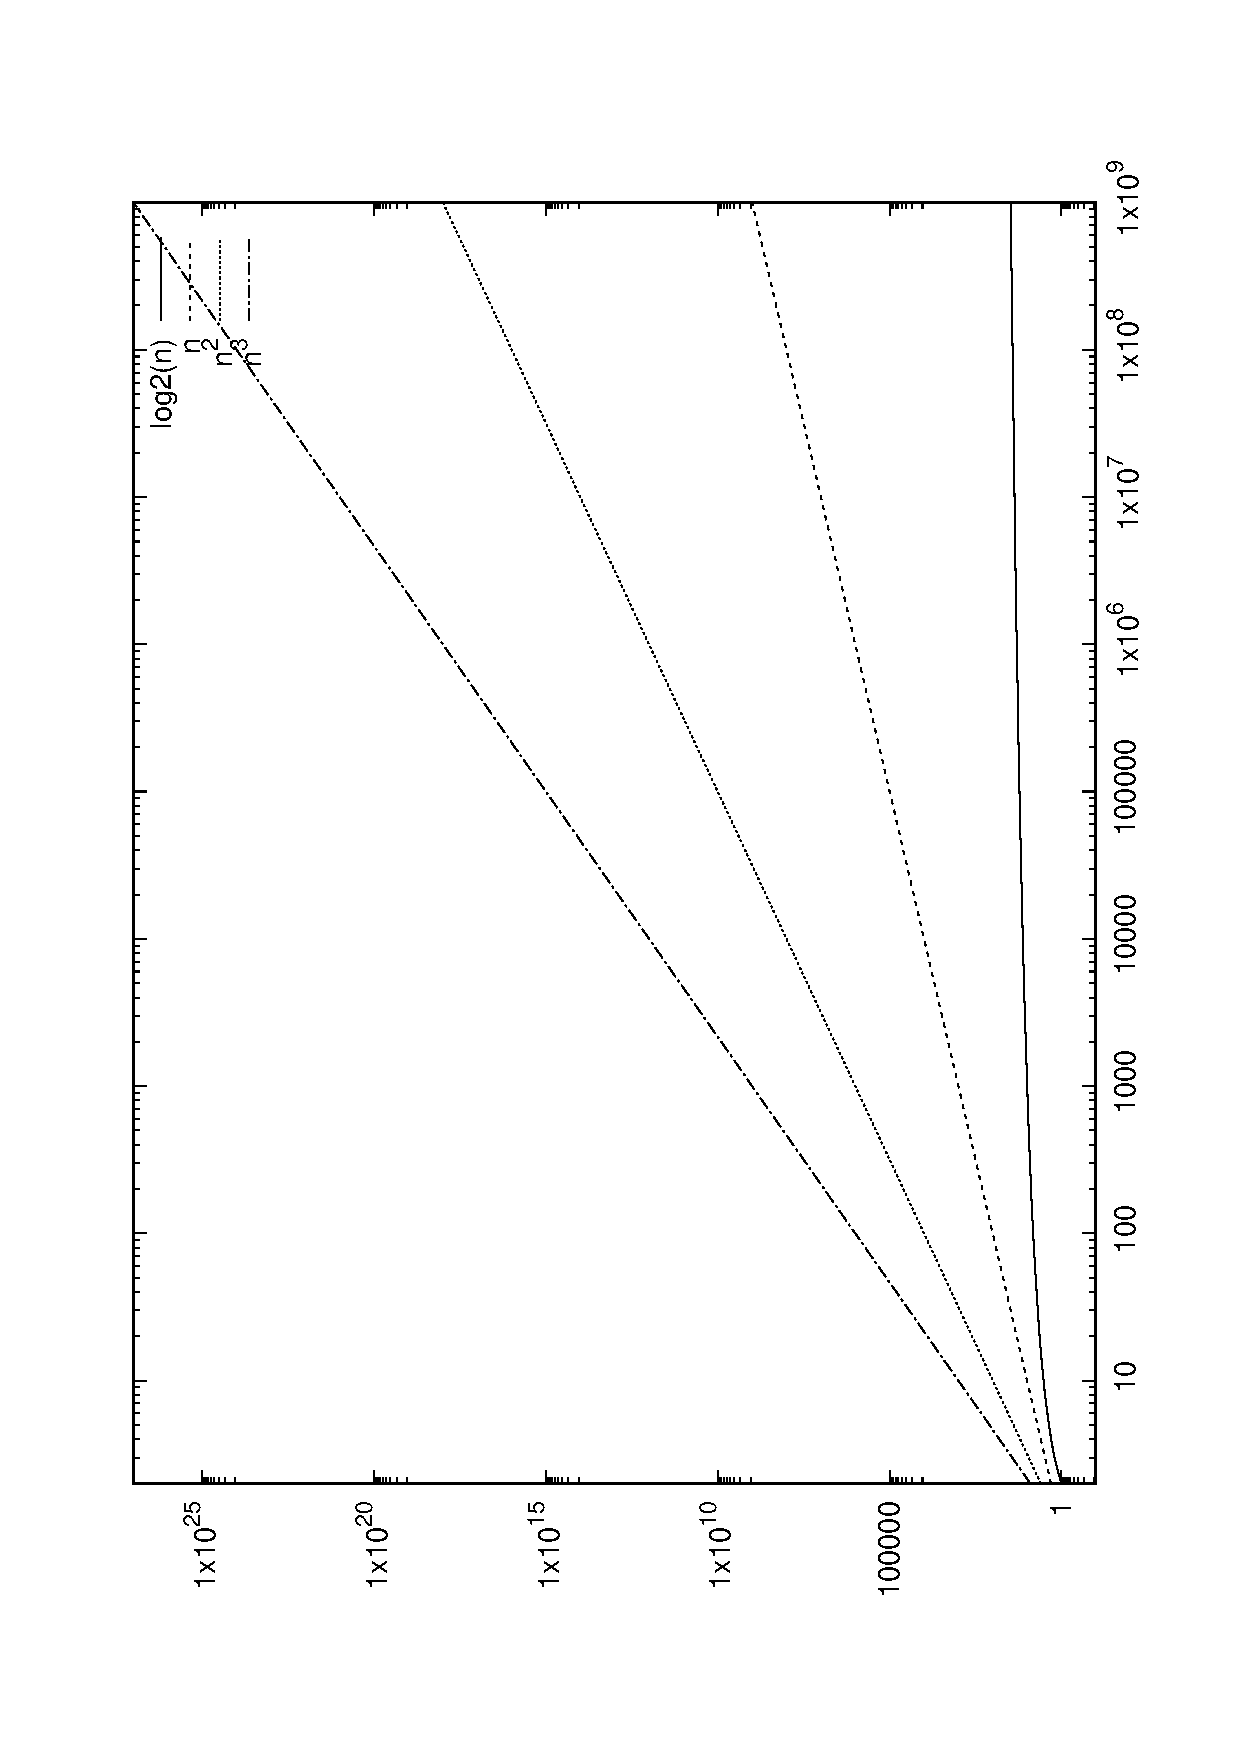
\includegraphics[width=.70\textwidth,angle=-90]{execution-time}
    \end{center}
  \end{frame}

  \begin{frame}{speedup}
    \begin{block}{speedup ($S=T_s/T_p$)}
      \begin{itemize}
        \item the ratio of time taken to solve a problem on a single processing
          element to the time required to solve the same problem on a parallel
          computer with $p$ processing elements
      \end{itemize}
    \end{block}
    \note[item] {Axpy --- $S=\Theta(\frac{n}{n/p})=\Theta(p)$}
    \note[item] {Reduction --- $S=\Theta(n/\log n)$}
    \note[item] {Matrix-vector --- $S=\Theta(n^2/n)=\Theta(n)$}
    \note[item] {Matrix-matrix --- $S=\Theta(n^3/n^2)=\Theta(n)$}
    \note[item] {What are the limits of speedup?}

    \vspace{-2ex}
    \begin{center}
      \only<2>{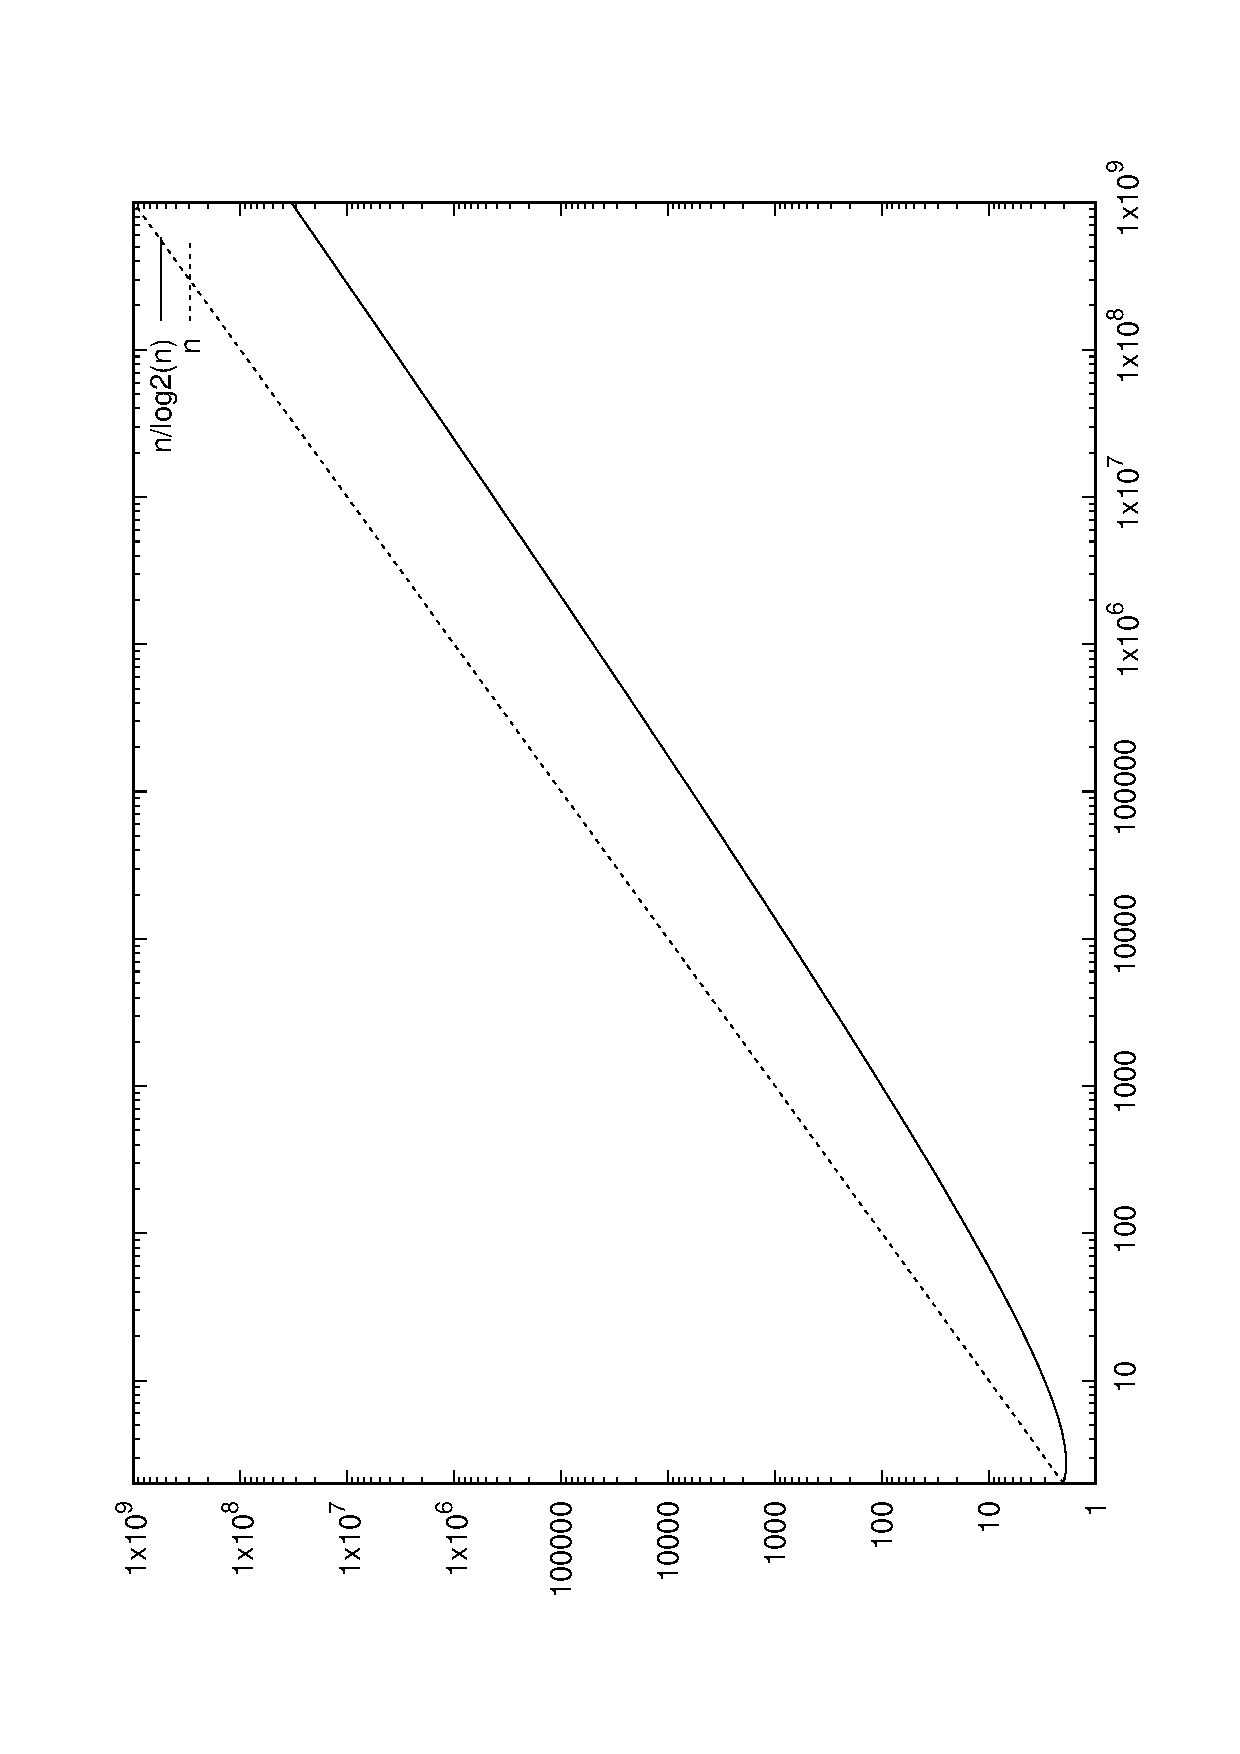
\includegraphics[width=.45\textwidth,angle=-90]{n-logn}}
    \end{center}
  \end{frame}

  \begin{frame}{Amdahl's law}
    Speedup is limited by the fraction of a parallel program that is serial.

    If $r$ is the fraction of the code which is serial, then

    \[
      S=\frac{T_s}{T_p}=\frac{T_s}{(1 - r) T_s/p + rT_s}
    \]

    \vspace{-2ex}
    \begin{center}
      \only<2>{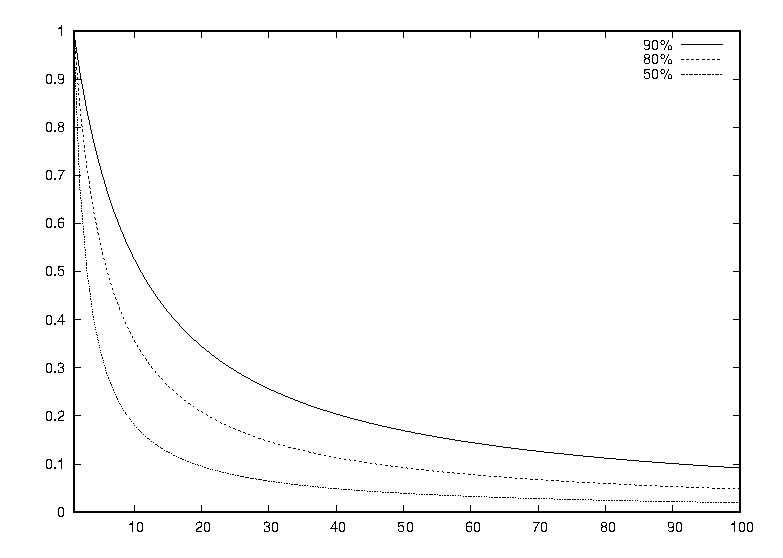
\includegraphics[width=.65\textwidth]{amdahl}}
    \end{center}

    \only<3->{In general, we cannot get a speed up better than
      \[
        \frac{1}{r}
      \]
    }
  \end{frame}

  \begin{frame}{efficiency}
    \begin{block}{efficiency ($E=S/p$)}
      \begin{itemize}
        \item the ratio of speedup to the number of processing elements --- the
          fraction of time for which a processing element is usefully employed
      \end{itemize}
    \end{block}
    \note[item] {Reduction --- $E=\Theta(n/\log n)/n=\Theta(1/\log n)$}
    \note[item] {Matrix-vector --- $E=\Theta(n)/n=\Theta(1)$}
    \note[item] {Matrix-matrix --- $E=\Theta(n)/n=\Theta(1)$}
    \note[item] {Why do you think that the efficiency of adding numbers is less
      than matrix-vector or matrix-matrix?}
    \note[item] {What are the limits of efficiency?}

    \vspace{-2ex}
    \begin{center}
      \only<2>{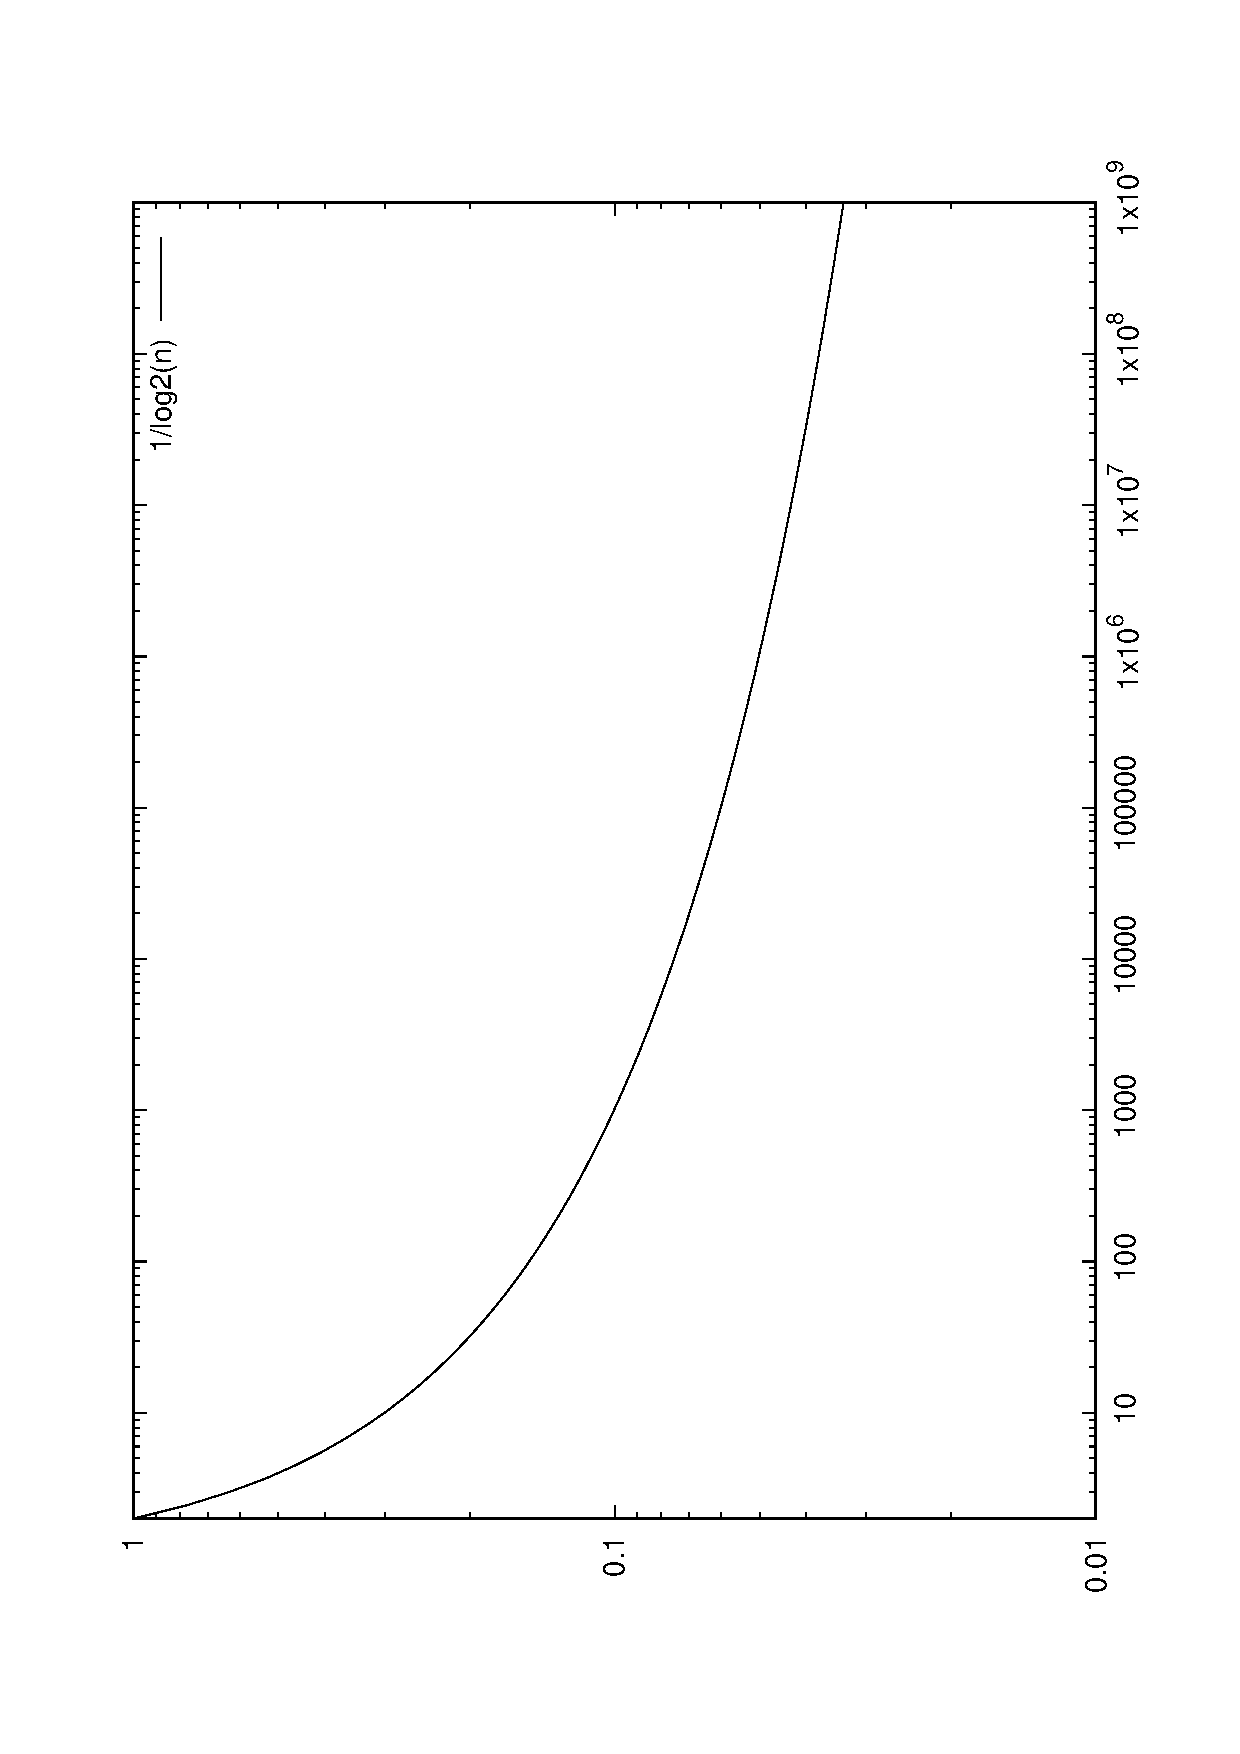
\includegraphics[width=.45\textwidth,angle=-90]{1-logn}}
    \end{center}
  \end{frame}

  \begin{frame}{cost}
    \begin{block}{cost ($C=pT_p$)}
      \begin{itemize}
        \item the sum of the time spent by all processing elements solving the
          problem
        \item \emph{cost-optimal} if $C=T_s$
      \end{itemize}
    \end{block}
    \note[item] {Axpy --- $C=\Theta(n)$}
    \note[item] {Reduction --- $C=\Theta(n\log n)$}
    \note[item] {Matrix-vector --- $C=n\times\Theta(n)=\Theta(n^2)$}
    \note[item] {Matrix-matrix --- $C=n\times\Theta(n^2)=\Theta(n^3)$}
    \note[item] {Reduction is not cost-optimal, the others are}

    \vspace{-2ex}
    \begin{center}
      \only<2>{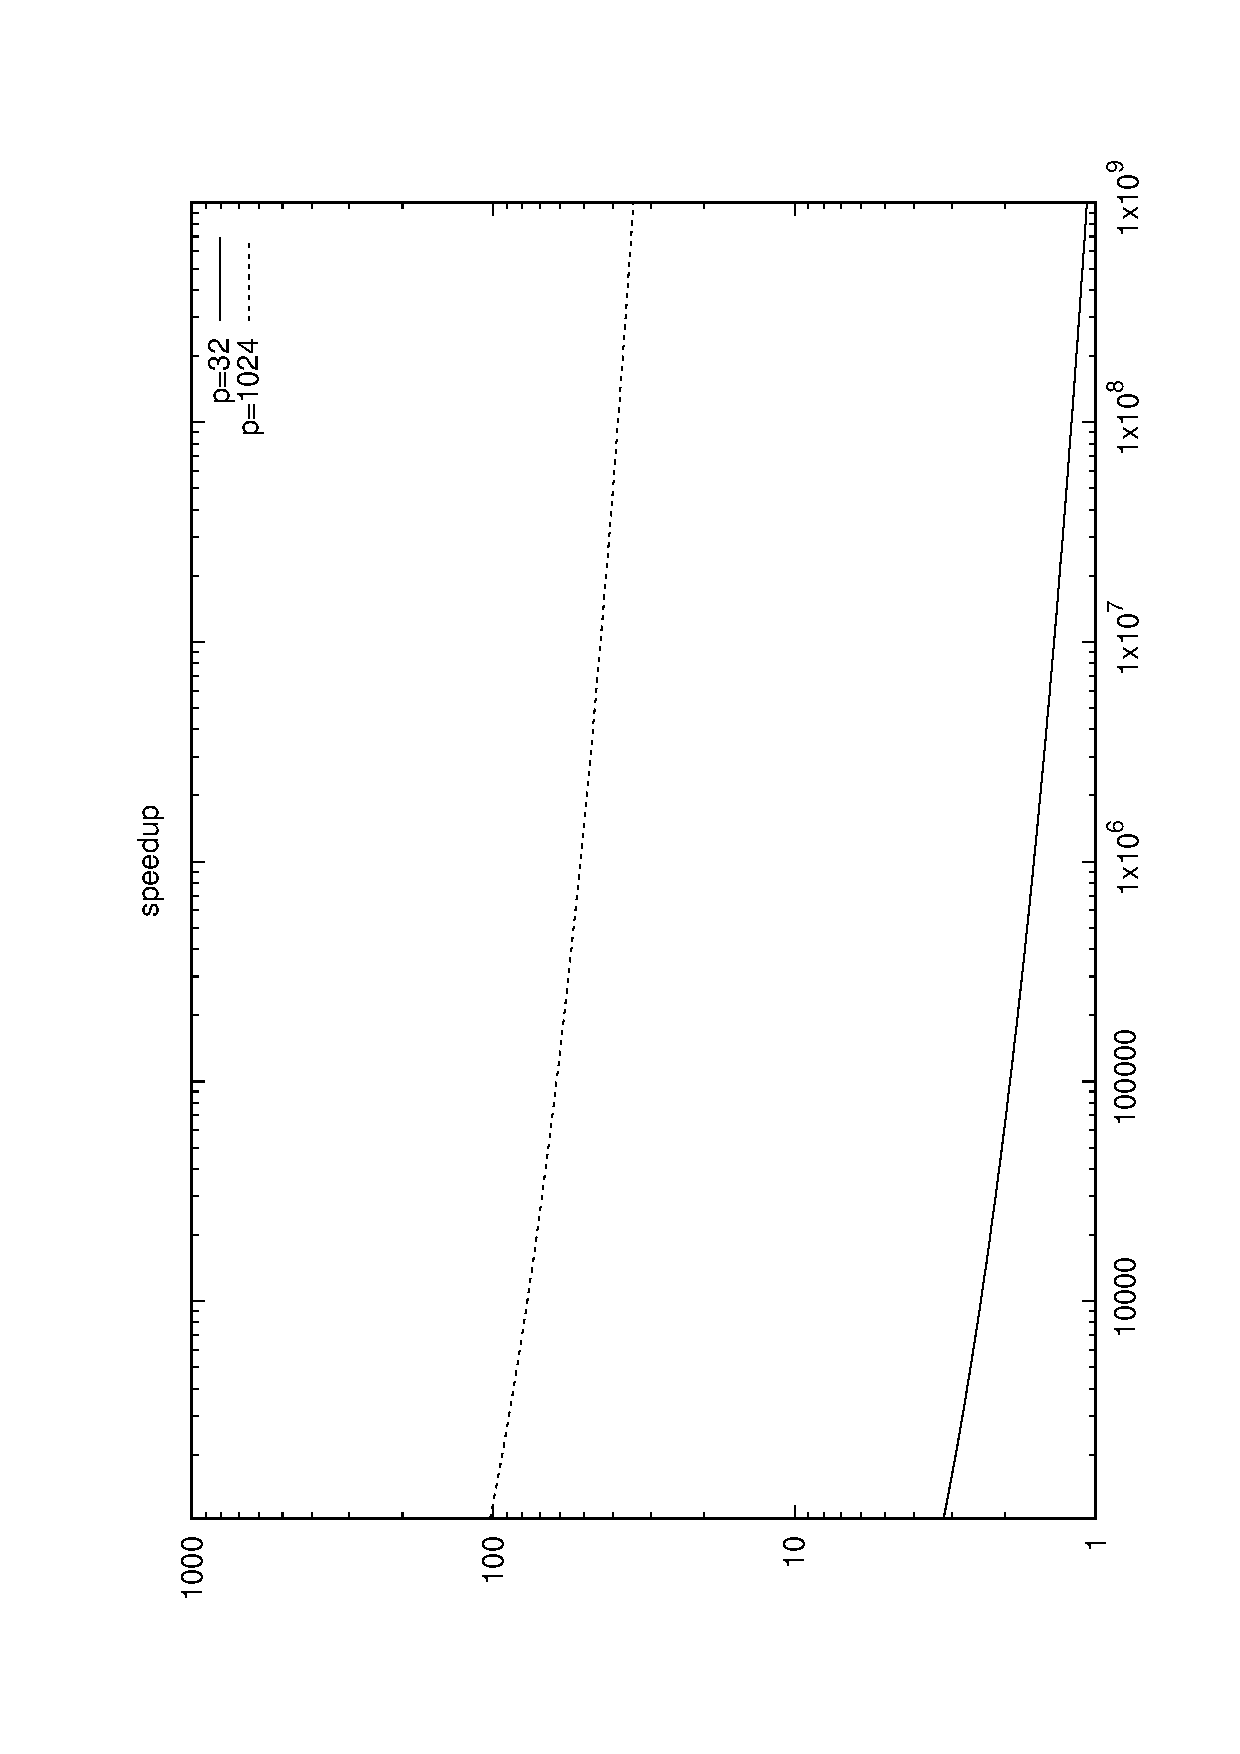
\includegraphics[width=.45\textwidth,angle=-90]{p-logn}}
    \end{center}
  \end{frame}

  \begin{frame}{exercise --- axpy}
    \begin{itemize}
      \item $T_p=?$
      \item $S=?$
      \item $E=?$
      \item $C=?$
    \end{itemize}
  \end{frame}

  \begin{frame}{exercise --- axpy}
    $p=n$ --- \emph{cost-optimal}
    \begin{itemize}
      \item $T_p=\Theta(n/p)$
      \item $S=\Theta(\frac{n}{n/p}=p)$
      \item $E=\Theta(1)$
      \item $C=\Theta(n)$
    \end{itemize}
  \end{frame}

  \begin{frame}{exercise --- reduction}
    $p=n$ --- \emph{not cost-optimal}
    \begin{itemize}
      \item $T_p=\Theta(\log n)$
      \item $S=\Theta(\frac{n}{\log n})$
      \item $E=\Theta(\frac{1}{\log n})$
      \item $C=\Theta(n\log n)$
    \end{itemize}

    $p>n$ --- too many processing elements, use less

    $p<n$ --- ?
  \end{frame}

  \begin{frame}{exercise --- reduction}
    \addtocounter{framenumber}{-1}
    $p=n$ --- \emph{not cost-optimal}
    \begin{itemize}
      \item $T_p=\Theta(\log n)$
      \item $S=\Theta(\frac{n}{\log n})$
      \item $E=\Theta(\frac{1}{\log n})$
      \item $C=\Theta(n\log n)$
    \end{itemize}

    $p>n$ --- too many processing elements, use less

    $p<n$ --- \emph{not cost-optimal?}
    \begin{itemize}
      \item $T_p=\Theta(\frac{n}{p}+\log p)$
      \item $S=\Theta(\frac{n}{\frac{n}{p}+\log p})$
      \item $E=\Theta(\frac{n}{n+\log p})$
      \item $C=\Theta(n+p\log p)$
    \end{itemize}
  \end{frame}

  \begin{frame}{exercise --- reduction}
    \addtocounter{framenumber}{-1}
    $p=n$ --- \emph{not cost-optimal}
    \begin{itemize}
      \item $T_p=\Theta(\log n)$
      \item $S=\Theta(\frac{n}{\log n})$
      \item $E=\Theta(\frac{1}{\log n})$
      \item $C=\Theta(n\log n)$
    \end{itemize}

    $p>n$ --- too many processing elements, use less

    $p<n$ --- \emph{cost-optimal iff $n=\Omega(p\log p)$}
    \begin{itemize}
      \item $T_p=\Theta(\frac{n}{p}+\log p)$
      \item $S=\Theta(\frac{n}{\frac{n}{p}+\log p})$
      \item $E=\Theta(\frac{n}{n+\log p})$
      \item $C=\Theta(n+p\log p)$
    \end{itemize}
    \note[item] {if you are given a problem size, what is the maximum number of
      processing elements that can be used in a cost optimal way?}
    \note[item] {what are the limits of efficiency\dots how about speedup?}
  \end{frame}

  %\begin{frame}<1>[label=countingsortalgorithm]{Counting sort}
  %  \begin{algorithmic}[1]
  %    \Function{CountingSort}{$inValues$,$outValues$}
  %      \State $count\gets \{0\}$
  %      \ForAll{$v$ \textbf{in} $inValues$}
  %        \State $count[v]\gets count[v]+1$
  %      \EndFor
  %      \State\Call{PrefixScan}{$count$}
  %      \ForAll{$v$ \textbf{in} $inValues$}
  %        \State $outValues[count[v]]\gets v$
  %        \State $count[v]\gets count[v]+1$
  %      \EndFor
  %    \EndFunction
  %  \end{algorithmic}
  %  \note[item] {Which of these steps can be parallelized?}
  %  \note[item] {Assuming we have $p=n$, and we can efficiently parallelize the
  %    two for loops, what is our analysis?}
  %  %\note<2>[item] {what are the limitations of this algorithm?}
  %\end{frame}

  %\begin{frame}{Counting sort --- analysis}
  %  $p=n$ --- ?
  %  \begin{itemize}
  %    \item $T_p=\Theta(\log |count|)$ or $T_p=\Theta(\log n)$
  %    \item $S=\Theta(\frac{n}{\log n})$
  %    \item $E=\Theta(\frac{1}{\log n})$
  %    \item $C=\Theta(n\log n)$
  %  \end{itemize}
  %  \note[item] {$T_p$ will be $\log |count|$ unless we use a dense
  %    data structure like a map in which case it will be $\log n$}
  %  \note[item] {$n$ will always be $\le |count|$}
  %\end{frame}

  %\againframe<2>{countingsortalgorithm}

  \appendix

  \begin{frame}[c]
    \begin{center}\ccbysa\end{center}

    except where otherwise noted, this worked is licensed under
    \href{http://creativecommons.org/licenses/by-sa/4.0/}{creative commons
    attribution-sharealike 4.0 international license}
  \end{frame}
\end{document}
